\documentclass[a4paper]{article}

\usepackage{geometry}
\usepackage{indentfirst}
\usepackage{amsmath,amssymb}
\usepackage{amsthm}
\DeclareMathOperator*{\argmax}{arg\,max}
\usepackage{amsthm}
\usepackage{bm}
\usepackage{bbm}
\usepackage{graphicx}
\usepackage{float}
\usepackage{color}
\usepackage{algorithm}
\usepackage{algorithmic}
%\renewcommand{\algorithmicrequire}{\textbf{Initialization:}}
%\renewcommand{\algorithmicensure}{\textbf{Inference:}}

\geometry{left=3cm,right=3cm,top=3.75cm,bottom=3.75cm}
\setlength{\parindent}{0em}
\setlength{\parskip}{1em}


\begin{document}

\newtheorem{thm}{Theorem}
\newtheorem*{thm*}{Theorem}
\newtheorem{lem}{Lemma}
\newtheorem{cla}{Claim}
\newtheorem{prop}{Proposition}

\title{Milestone 3 Report}

\author{Lei Zhong, Hantian Zhang, Jian Zhang}
\date{}
\maketitle

\abstract{}

\section{Data model}
    In this milestone, we use the full \cite{GHCN-D} dataset, which provides weather information from 1763 to 2014. 
    We use Amazon Web Services to run our program, \cite{boto} is a Python interface to it. We upload all the data to a bucket in \cite{S3}. Since a single file can exceed $1$GB, we divide the data into chunks of size of $50$M.
    The 1763 dataset is only $25$KB, so that we have to identify all the missing values, later when creating feature, replacing them with specific ones.

\section{The System Architecture}

\subsection{Description of the Architecture and Tools used}
As is shown in Figure \ref{fig:archi}, CLUE has four main steps : Feature Extraction, Sampling, Clustering and Visualization. The tools we use includes Amazon Elastic MapReduce\cite{EMR}, Scikit-learn\cite{sklearn} library and Google Map API\cite{GoogleMap}. The four steps are illustrated in details in the followling part.
\begin{figure}[htbp]
				\centering
				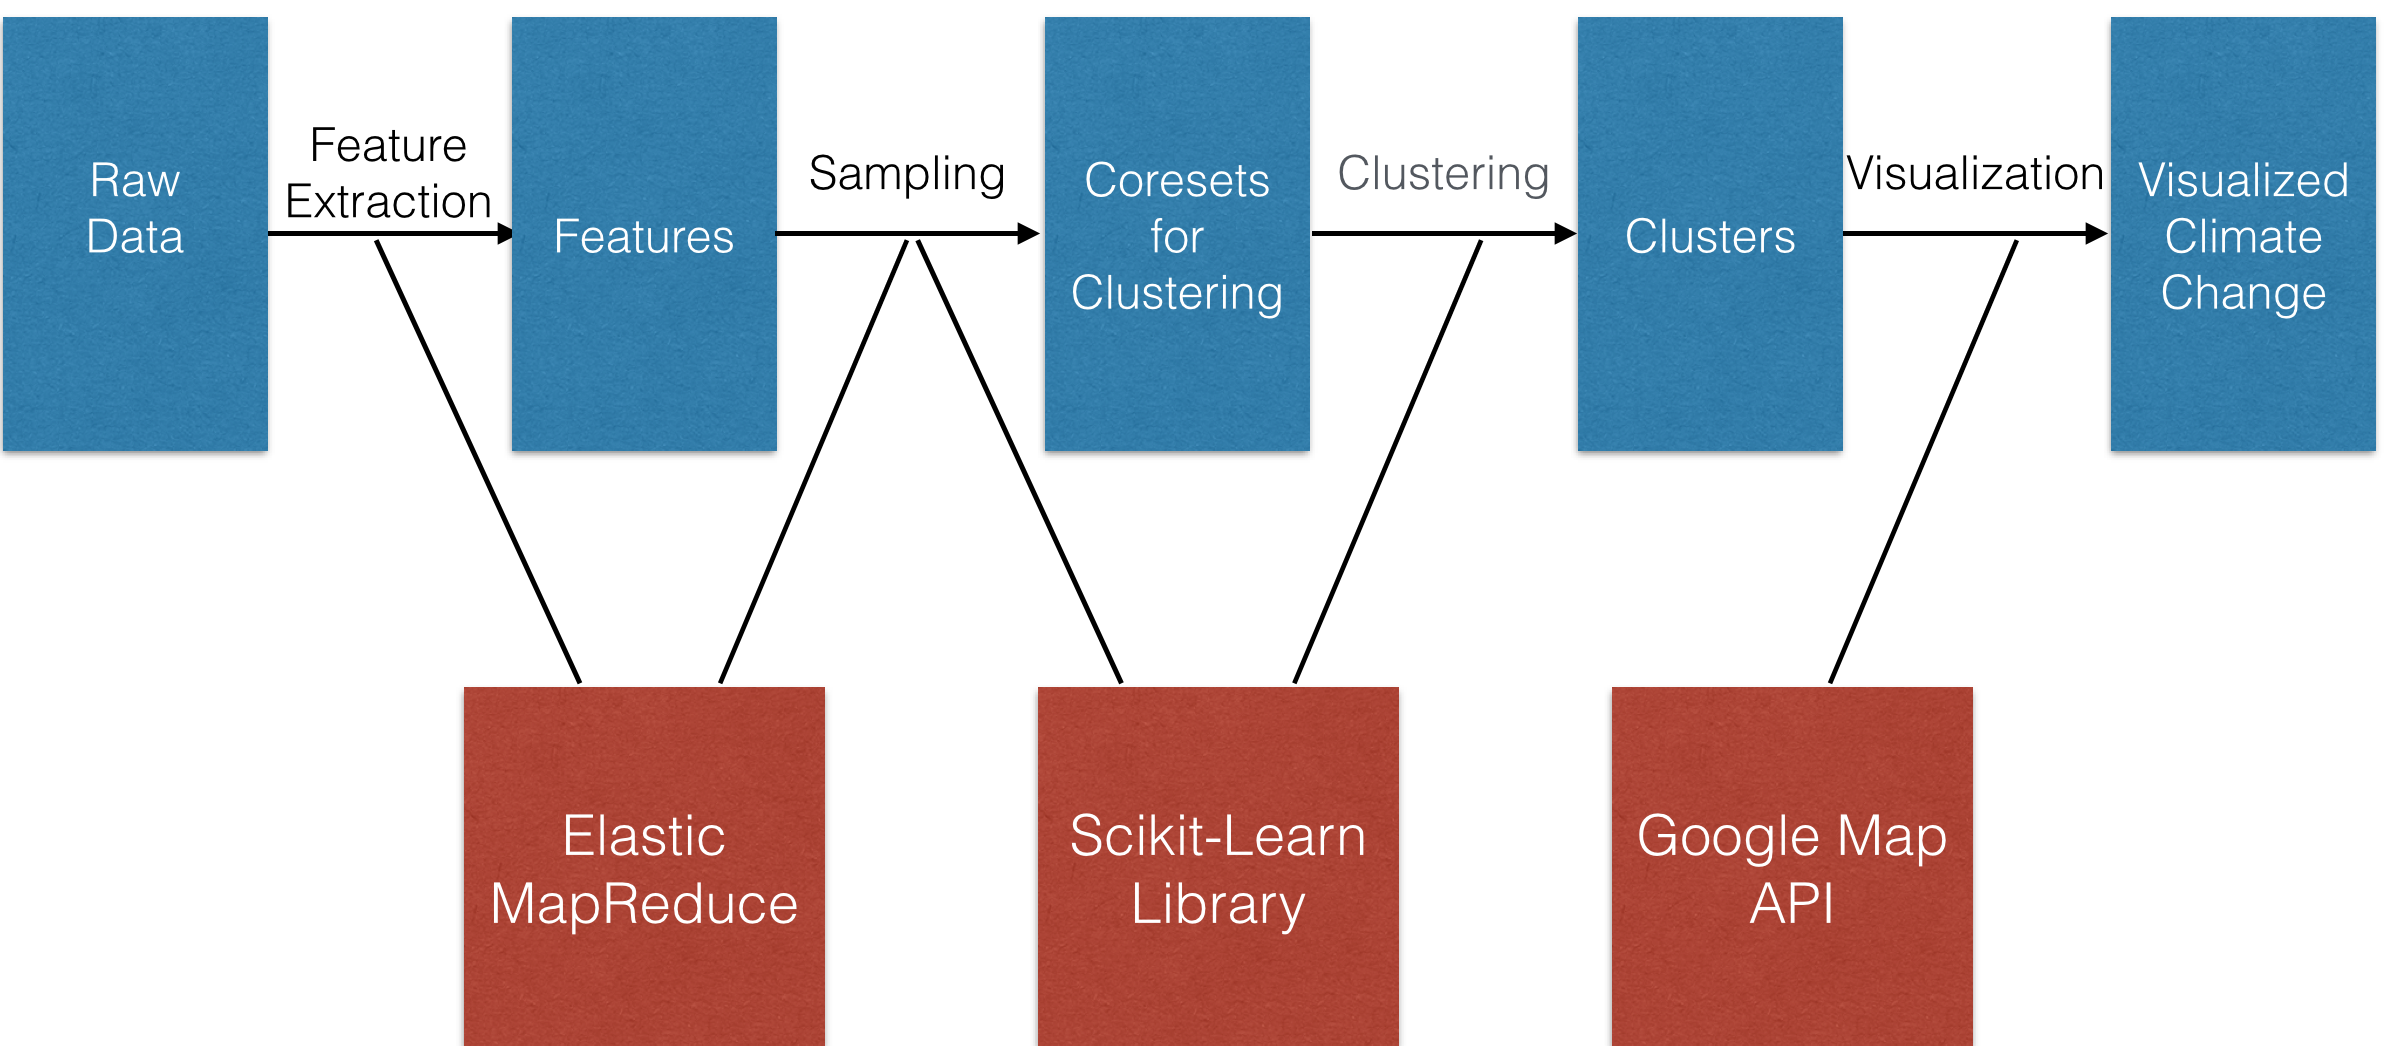
\includegraphics[width=0.9\textwidth]{images/Architecture.png}
				\caption{Architecture of CLUE}
				\label{fig:archi}
 \end{figure}
 
\subsubsection{Feature Extraction}
The raw data includes the climate data from 1763 to 2014, the total volume of raw data is about 100 Gigabytes, which is too big to fit in the memory. So we use Amazon Elastic MapReduce to calculate features. We use the same features setting with the previous milestone. The feature extraction consists of 3 sub-steps, including calculating features for existing data, filling in the missing value using the mean value of the feature value of all other existing data and normalizing data. Each of these sub-steps is done by a map-reduce task because of the huge volume of data. Through feature extraction, we get about 300 million 60-dimentional data points.

\subsubsection{Sampling}
We want to use all data points to run clustering. However, we use the k-means function in the scikit-learn library to compute clusters. It is impossible for that k-means function to run on 300 million of data points. We have two choices of handling this. One is to write a parallel k-means function that can run on Amazon EMR, the other one is to sample these data points so that the sample points are able to represent all the data points with the minimum loss of information. We choose the second approach and use coreset for k-means clustering. The coreset is a set of data points that is used to run the weighted k-means clustering. Each point in the coreset represents some original data points that are near to it. These data points are assigned the same label as the point in the coreset. The coreset sampling is done by an iterative step, where in each step, we uniformly sample some data points, calculate distance to the nearest point in the sampling set for every data point, remove data points whose distance to the nearest point in the sampling set are below median. Iterate this step until the number of remained data points is smaller than a pre-defined number and we get a coreset sampling of data. In addition to coreset sampling, we could also run the clustering on the whole data for a couple of years for detailed information in these years, which is done in milestone 2.


\subsubsection{Clustering}
Having the coreset whose size is reasonable, we can run weighted k-means algorithm on the coreset and calculated all the centroids. The last step is to assign each data point to the nearest centroid and give that data a label. This step is also done by a map-reduce task.

\subsubsection{Visualization}
For the visualization part, we used the same technique that we have used in milestone 2. We used Google Map API to visualize the clustering result. For each year, all the stations in that year are placed on the map according to its location and the stations in the same cluster have the same color. We did an animation to show the change of clusters that reflects climate change.

\subsection{Limits in Scalability and Possible Improvements}
We have used most data that is available, however, due to the sampling process, the pattern of the result of clustering is not as obvious as the previous milestone. The main limit is the scalability of the clustering algorithm. I think coreset sampling is a good way to handle this, but due to the time limit, the coreset sampling we implemented has a lot of room for improvement and the clustering result is not as good as imagined. We would like to improve our sampling method and try different parameters for better sampling and clustering result. Also, we would like to write a parrallel k-means algorithm so that we can use more data points if possible.

\section{Result of the Implementation}
\subsection{Quality Measures and Interpretation}
\begin{figure}
    \centering
    \begin{tabular}{c}
        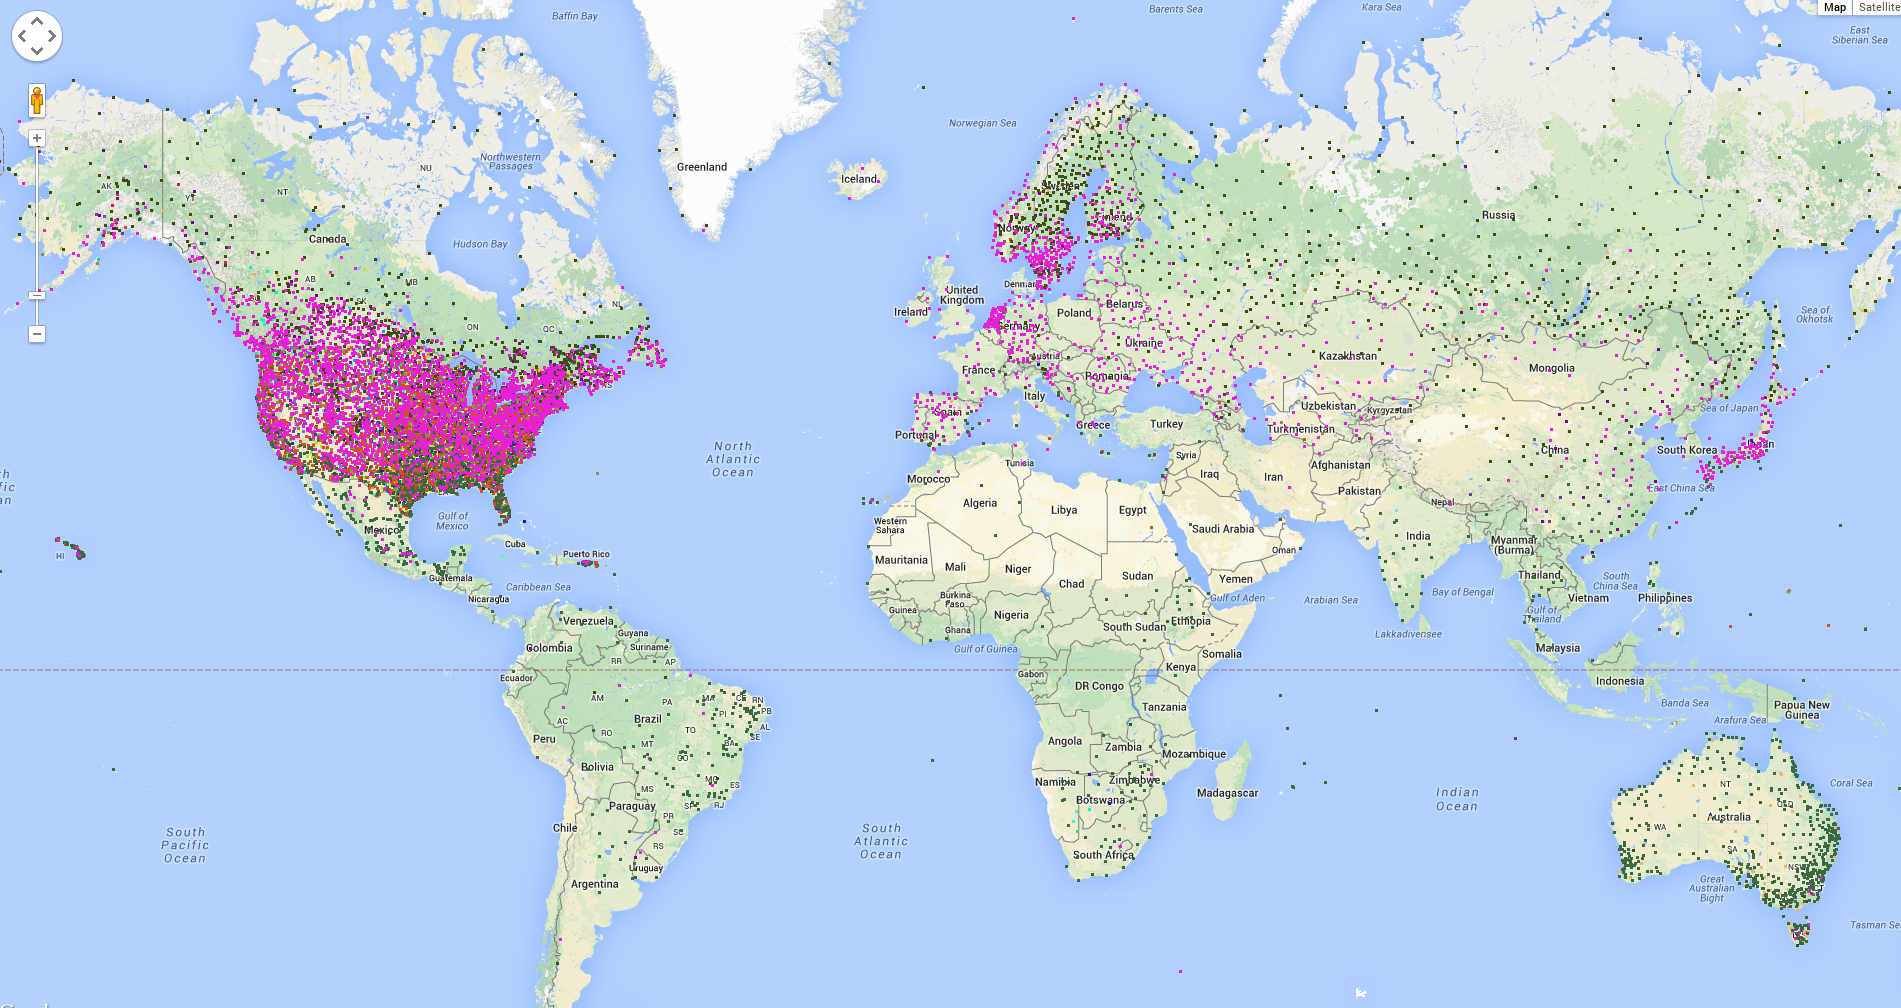
\includegraphics[width =.65\linewidth]{figure/1983.png}\\         1983 \\
        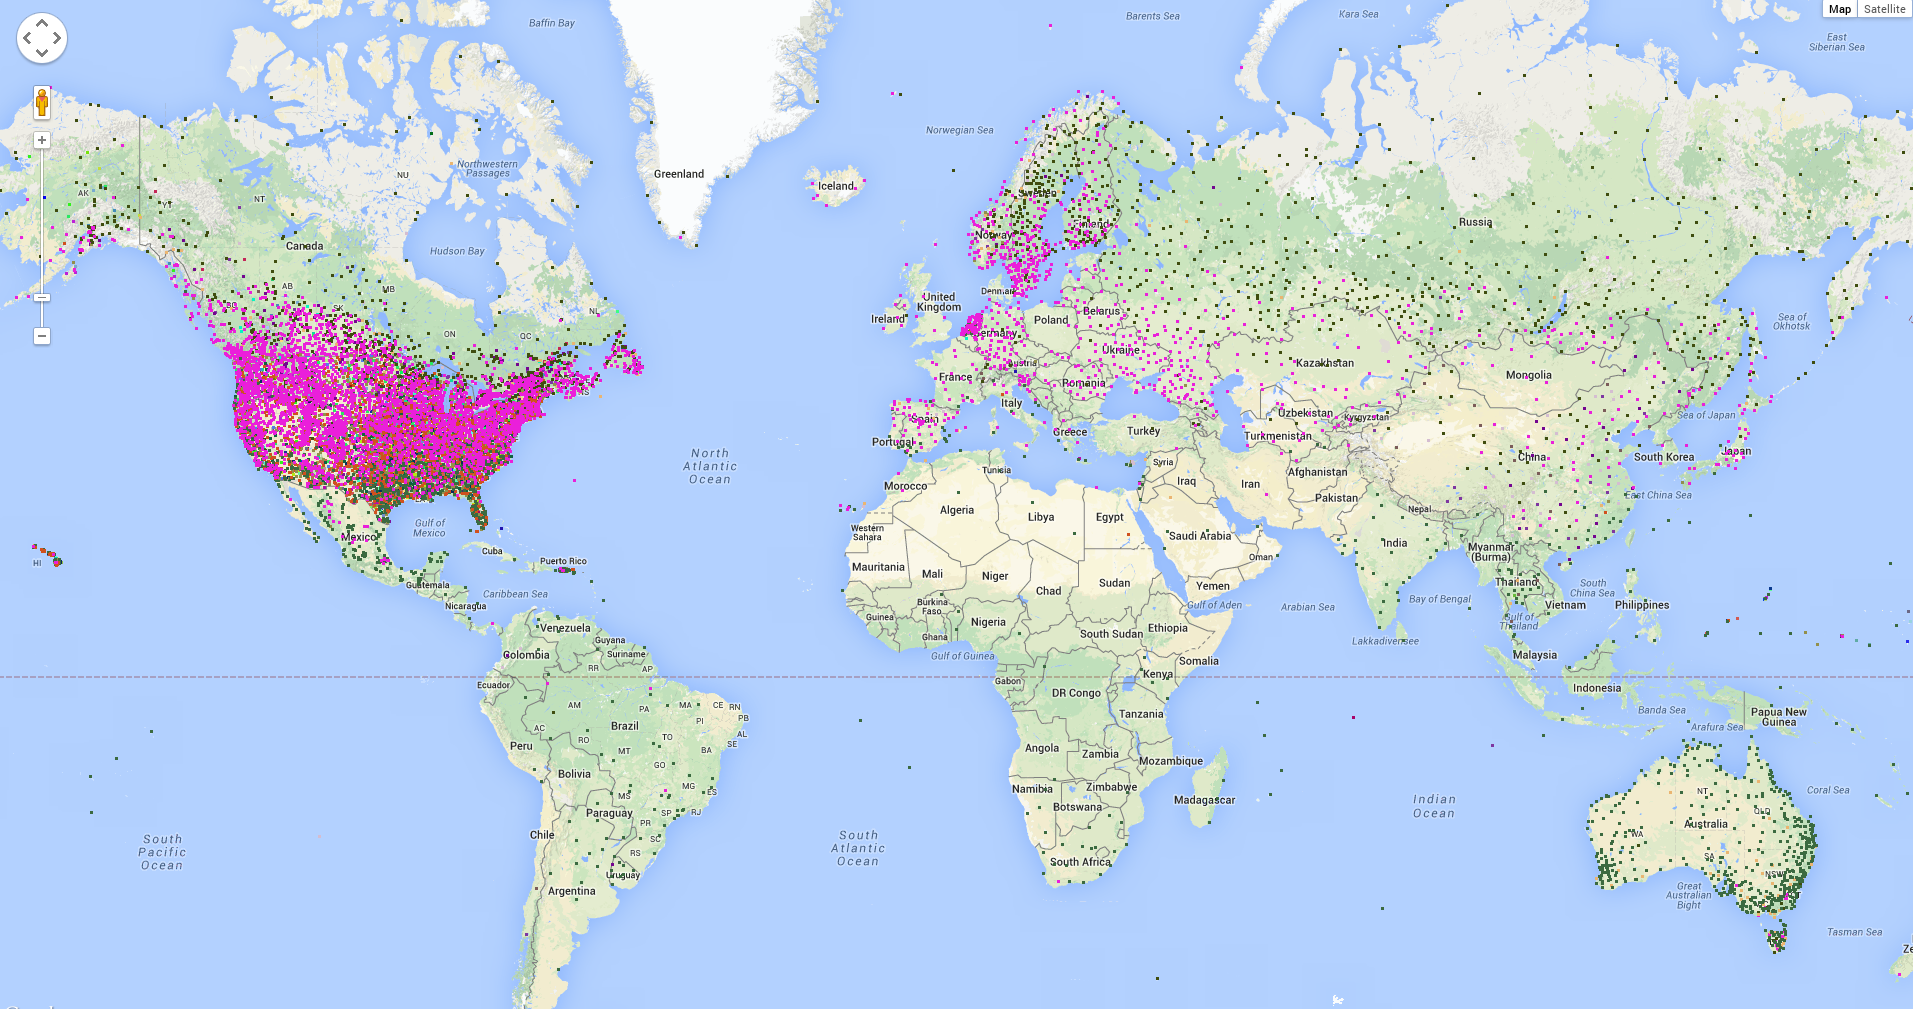
\includegraphics[width =.65\linewidth]{figure/1993.png} \\
        1993 \\
        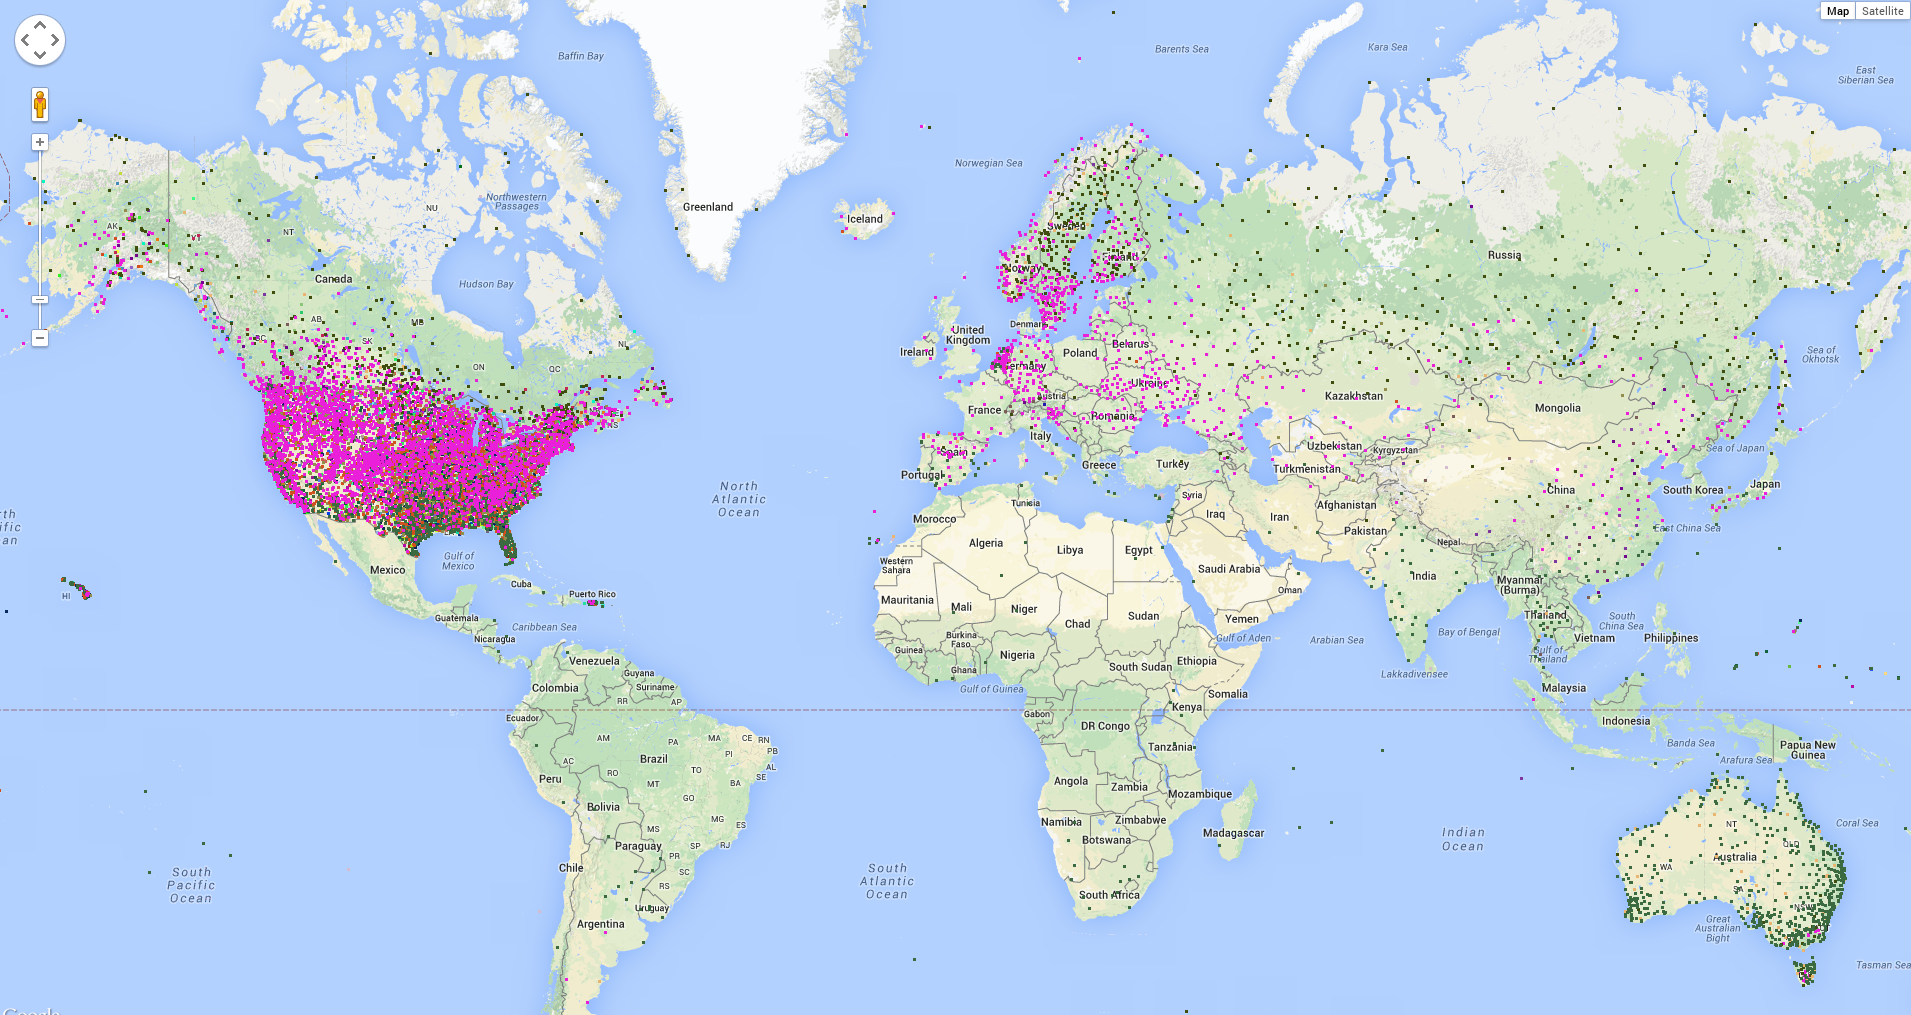
\includegraphics[width =.65\linewidth]{figure/2003.png} \\         2003 \\
        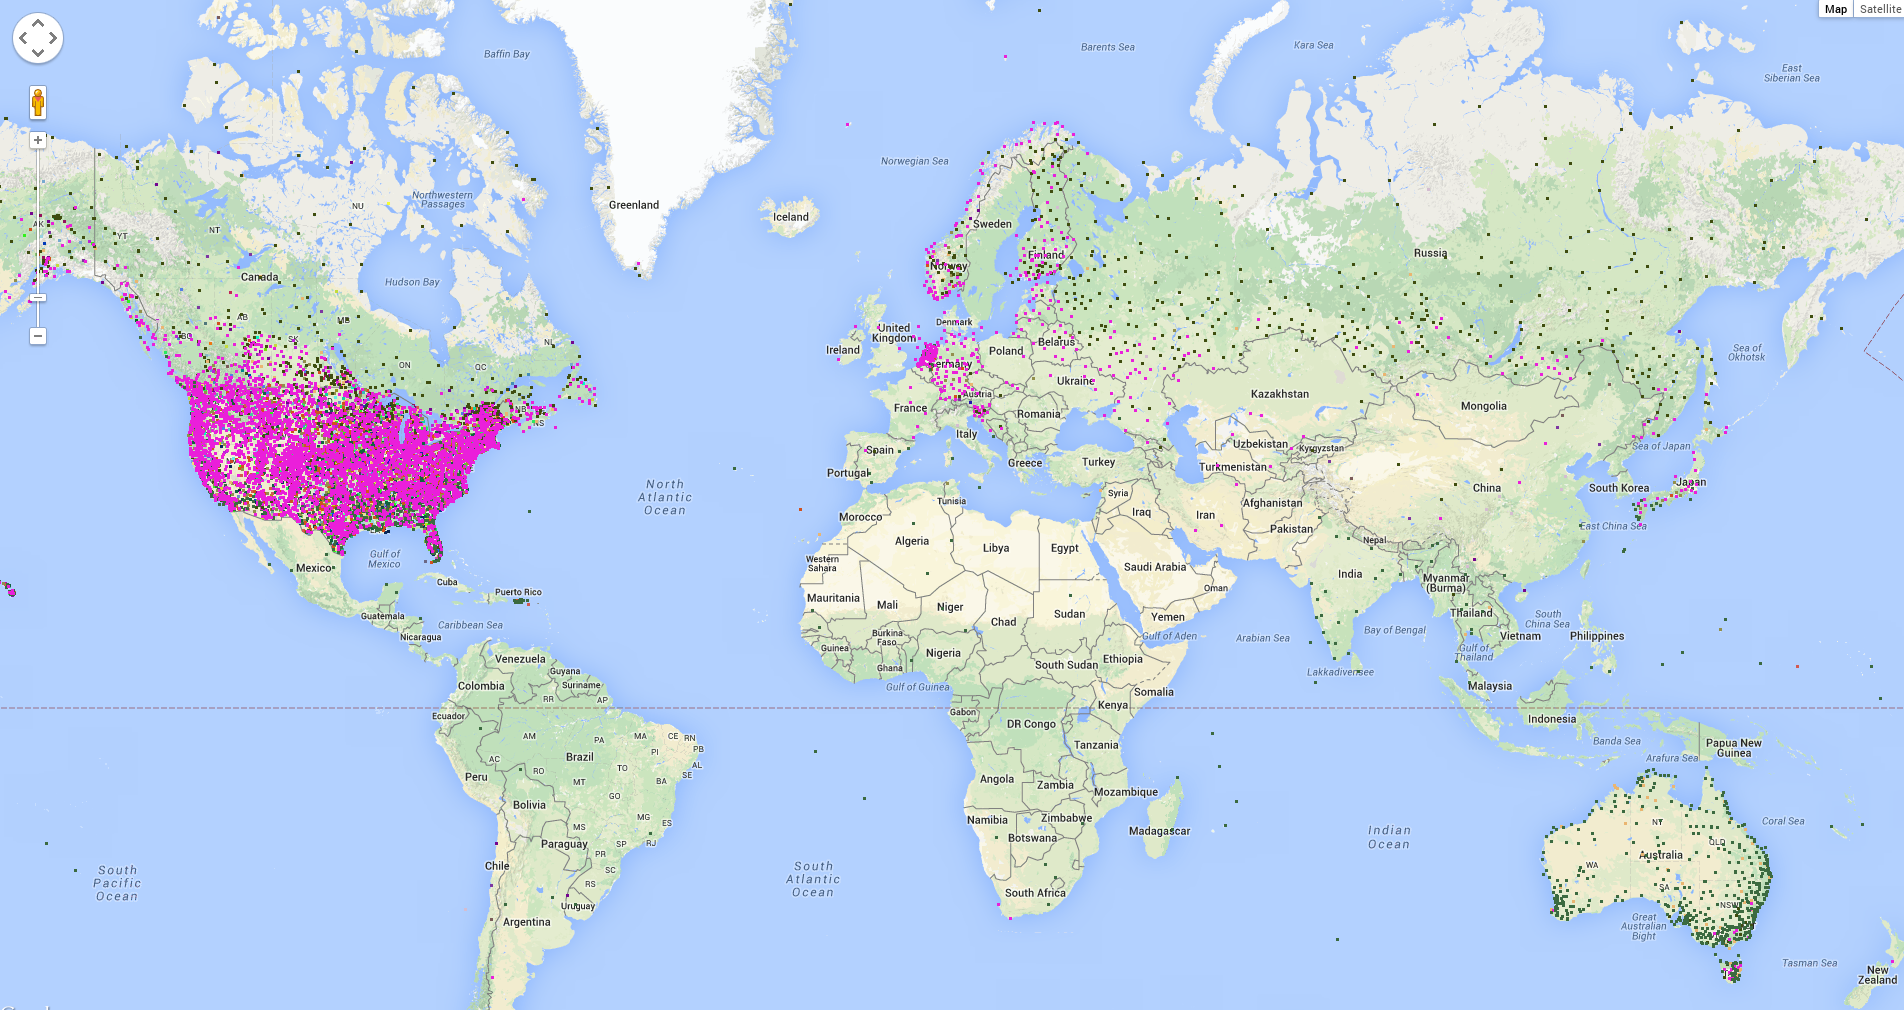
\includegraphics[width =.65\linewidth]{figure/2013.png} \\
        2013\\
    \end{tabular}
    \caption{Clustering results of different years.}
    \label{fig:ClusteringFlow}
\end{figure}

From the clustering flow spanning over 4 decades in Fig \ref{fig:ClusteringFlow}, we are still not satisfied with the current results. In the following, we will discuss a few aspects of the visualization, as well as analysis with possible solutions in the next stage.

From the results, we can see there are only 3 big clusters (Majority of North America, Asia and Russia, Region around Florida) even if we set the number to be 300 for Kmeans. It does not align well with our prior geology knowledge and expected results. There are several possible reasons for this results:

1. We are eliminating data points whose features have relatively large number of missing values. Our threshold might be improper right now. For example, we can observe few points in China while there do exists much more data points in the raw data. It exerts the potential risk of removing possible climate clusters where monitoring data are not complete in all of the five measurements.

2. As we employ uniform sampling to generate coreset, we are still making efforts to analyse 2 specific distributions: (1) distribution of  numbers of data points represented by each coreset point. (2) distribution of numbers of data points represented by each cluster in coreset. If this distribution is close to uniform distribution, it means points in coreset represent unbalanced neighborhood. Then we can conclude our sampling strategy might be improper. We will adjust our sampling strategy and parameters to improve the result quality before the next milestone.

However, there are also some encouraging points in the current results. From the flow from 1983 to 2013, we can observe the three biggest clusters covering roughly the same areas with minor difference. It is a good indication that similar year-wise climate patterns are clustered into the same cluster.

We will make efforts in verifying the correctness of sampling strategy, validity of features and different parameter. We expect better results before the last milestone.

\subsection{Scalability}
For our feature generation tasks, we employ the following EMR master-slave pair for computation. A m3.2xlarge machine with 8 cores and 30GB memory is deployed as the master server, 2 m1.xlarge machines with 4 cores and	15GB memory are employed as slave clients. The running time and peak memory consumption for different feature generation task is summarized in the following table.

\begin{table}[H]
    \begin{tabular}{| c | c | c | c |}
    \hline
    Task & running time & peak memory & normalized instance hour \\
    \hline
    \hline
    Extract feature with missing value & 3h45min & 25GB & 124h\\
    \hline
    Calculate mean and variance of features & 40min & 25GB & 31h\\
    \hline
    Fill missing values and normalize features & 3h47min & 25GB & 124h\\
    %\hline
%    Recalculating mean and variance for normalization &  &  &\\
%    \hline
%    Feature normalization &  &  & \\
    \hline
    \end{tabular}
    \caption{Scalability performance of tasks related to feature generation.}
    \label{tbl:PerfTable}
\end{table}

As we meet difficulties in installing scikit learn library with bootstrap script when launching clusters. We set up Hadoop 2.5.2 environment on a local machine with a quad-core i5-4570 3.2Ghz processor and 16 GB memory. To meet the memory requirement for running intensive tasks, we set up the hadoop mapper and reducer memory at \textit{mapred-site.xml } as the following snippet shows.

\begin{lstlisting}
<configuration>
    <property>
        <name>mapred.job.tracker</name>
        <value>localhost:54311</value>
    </property>
    <property>
        <name>mapreduce.map.memory.mb</name>
        <value>4096</value>
    </property>
    <property>
        <name>mapreduce.reduce.memory.mb</name>
        <value>8192</value>
    </property>
    <property>
        <name>mapreduce.map.java.opts</name>
        <value>-Xmx3072m</value>
    </property>
    <property>
        <name>mapreduce.reduce.java.opts</name>
        <value>-Xmx6144m</value>
    </property>
</configuration>

\end{lstlisting}


%\bibliographystyle{plain}
%\bibliography{Proposal}
\begin{thebibliography}{1}
    \bibitem{GHCN-D} Peterson, Thomas C., and Russell S. Vose. ``An overview of the Global Historical Climatology Network temperature database.'' Bulletin of the American Meteorological Society 78.12 (1997): 2837-2849.
    \bibitem{boto} https://boto.readthedocs.org/en/latest/
    \bibitem{S3} http://aws.amazon.com/de/s3/
\end{thebibliography}

\end{document}
